\section{Libraries Design}

% Details on implementation.
% Architecture.

% TODO:
% - stunning architecture diagram
% - exciting example of usage
% - unbelievable python API showcase

Implemented sparse boolean linear algebra libraries for NVIDIA Cuda and OpenCL platforms  are called \textit{cuBool} and  \textit{clBool} respectively.
%%%%% I think, this info is too excessive. If you want to know something, go to the page with repos
% The projects are hosted on GitHub.
% The source code is licensed under MIT license.
% The build process is straightforward: it is configured with CMake tool and requires extra setup only for platform-specific development kits.
The architecture of the libraries is depicted in figure~\ref{fig:generic_architecture}.
The core of the libraries is written in the C++ programming language, which is well-suited for performance and resource critical computational tasks.
The GPU related logic is in the platform specific backends: Cuda and OpenCL, which use respective technologies for resources and GPU executable code management.
The cuBool library exposes C compatible API, which gives expressiveness and allows one to embed that API into other execution environments by interoperability mechanisms.
Pycubool module encapsulates such functionality and provides it for the high-level Python runtime.

It is worth to mention, that it is convenient to create the single library with common interface and several backends for different execution targets.
At this time clBool and cuBool are distinct libraries, but they can be integrated into a single library.
This integration is planned for the near future.
This process requires careful selection of the interface to allow the end user to properly configure the library for specific tasks, as well as to provide the option to automatically select a specific implementation depending on the capabilities of the target device.

\begin{figure}[t]
    \centering
    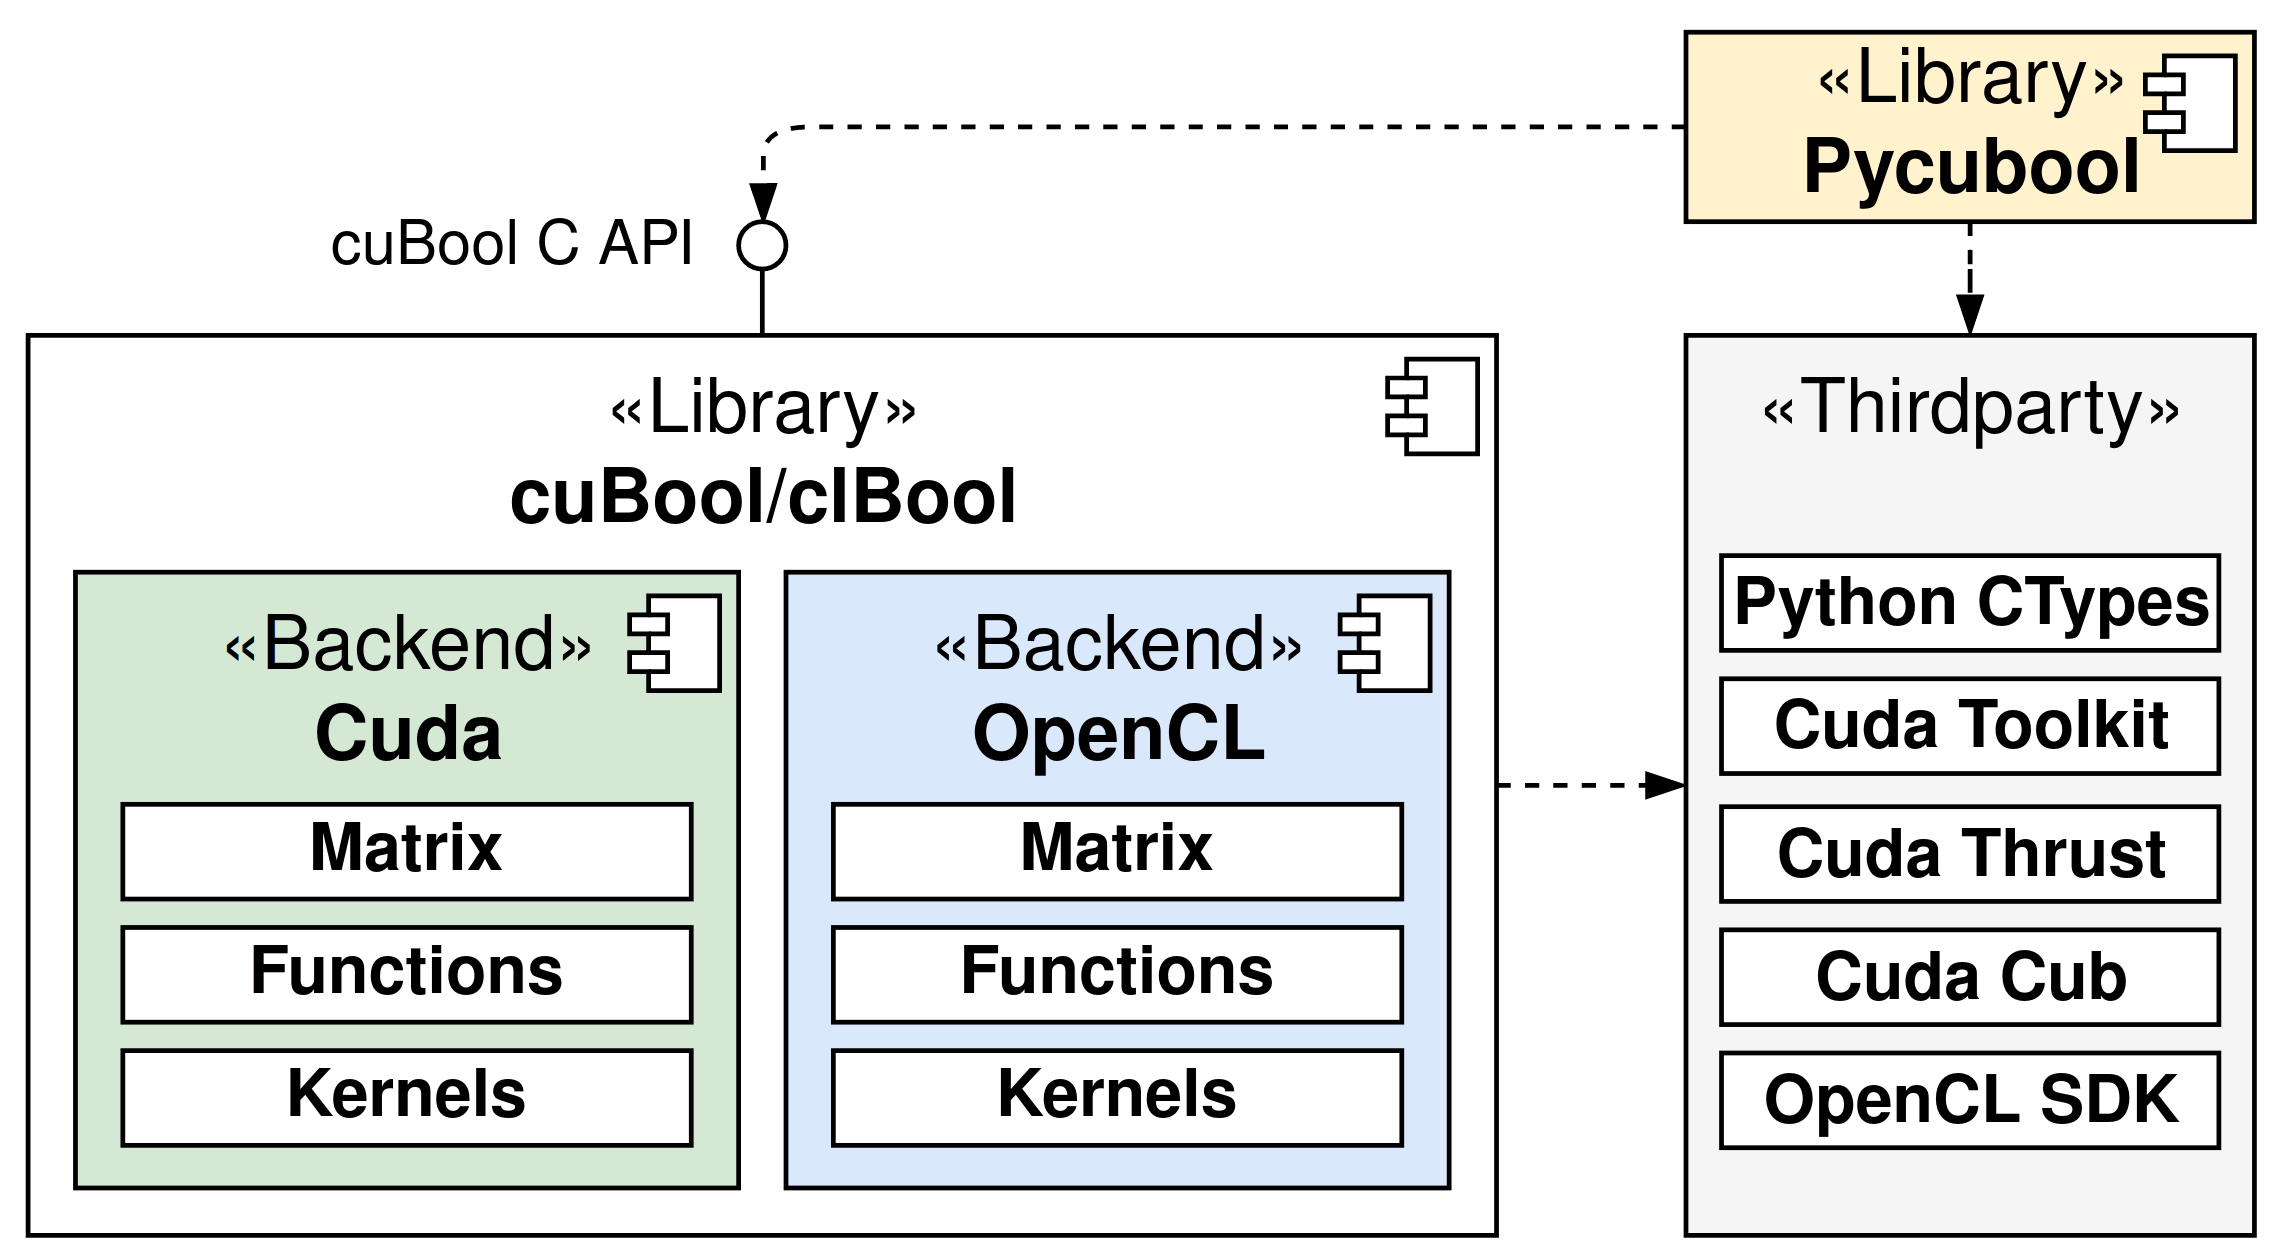
\includegraphics[width=0.39\textwidth]{generic_architecture.png}
    \caption{Sparse Boolean linear algebra libraries architecture.}
    \label{fig:generic_architecture}
\end{figure}

Libraries operate on the boolean semiring with values set \{\textit{true}, \textit{false}\} with \textit{false} as an identity element, '$+$' operation is defined as logical \textit{or} and '$\times$' is defined as logical \textit{and}.
Values are also denoted as $\{1,~0\}$ respectively, and the abbreviation $\textit{nnz(M)}$ gives the number of non-zero cells of the matrix $M$.

The main primitive is a sparse matrix of boolean values, stored in one of the sparse formats.
The sparse vector is partially presented. 
Its full support will be added in the future. 
All available operations and functions are the following.

% \begin{itemize}
%     \item Create sparse matrix $M$ of size $m \times n$.
%     \item Delete sparse matrix $M$ and free all its internal resources.
%     \item Fill the matrix $M$ with values $L = \{(i,j)_k\}_k$. The result of this operation is $M_{i,j} = 1$ for each $(i, j) \in L$, and $M_{i,j} = 0$ otherwise.
%     \item \cho{Read matrix $M$ values $L = \{(i, j)~|~M_{i,j} = 1\}$.}
%     \item Matrix-matrix multiply-add operation $C \mathrel{+}= M \times N$.
%     \item Matrix-matrix add operation $M \mathrel{+}= N$.
%     \item Matrix-matrix Kronecker product $K = M \otimes N$.
% \end{itemize}

\begin{itemize}
    \item Create sparse matrix $M$ of size $m \times n$.
    \item Delete sparse matrix $M$.
    \item Fill matrix with values $\{(i,j)_k\}_k$.
    \item Read matrix values $\{(i, j)~|~M_{i,j} = 1\}$.
    \item Transpose $M = N^T$
    \item Sub-matrix extraction $M = N[i..m, j..n]$
    \item Matrix-vector reduce $V = \textit{reduceToColumn}(M)$
    \item Matrix-matrix multiplication $C \mathrel{+}= M \times N$.
    \item Matrix-matrix element-wise addition $M \mathrel{+}= N$.
    \item Matrix-matrix Kronecker product $K = M \otimes N$.
\end{itemize}